\documentclass[11pt]{article}
\usepackage[margin=1in]{geometry}
\usepackage{graphicx}
\usepackage{hyperref}
\usepackage{longtable}
\usepackage{amsmath}
\usepackage[section]{placeins}
\hypersetup{pdftitle={Homework 3 Track B: Q1 Q2 Q3 Q4 Q5 Q8 - 105 points},pdfauthor={Varunaditya Venkatesan}}
\title{Homework 3 --- Track B\\Q1, Q2, Q3, Q4, Q5, Q8 --- 105 points}
\author{Varunaditya Venkatesan}
\date{November 6, 2026}
\begin{document}
\maketitle
\begin{center}\textbf{Measured comparisons; inference limits stated explicitly}\end{center}
\noindent Selected exercises: \textbf{Q1, Q2, Q3, Q4, Q5, Q8 --- 105 points}.
\begin{center}
\begin{tabular}{llrl}
Question & Task & Points & Project status\\\hline
Q1 & Confirm pipelining & 10 & Measured comparisons\\
Q2 & Confirm out-of-order execution & 10 & Measured comparisons\\
Q3 & Confirm branch prediction & 10 & Measured comparisons\\
Q4 & Reverse engineer ROB size & 30 & Completed; preserved\\
Q5 & Integer GPR physical register capacity & 35 & Pressure bound measured\\
Q8 & Additional cost of a TLB miss & 10 & Native cost qualified\\\hline
 & Total & 105 & Q6 dropped
\end{tabular}
\end{center}
\noindent Implementation order: Q3 $\rightarrow$ Q1 $\rightarrow$ Q2 $\rightarrow$ Q5 $\rightarrow$ Q8.
Native measurements now cover both machines for all six selected questions; applicable hardware-enclave comparisons use Artemisia. The missing Charnwood Q4 comparison was added with unchanged preserved source, without rerunning Artemisia Q4. Q5 reports a qualified speculative destination-pressure bound, not an invented total PRF size. Q8 enclave miss-class attribution remains unqualified. Functional smoke checks are kept separate from performance evidence.
\clearpage
\section{Machines and common protocol}
Charnwood uses an Intel Core i7-6700 (Skylake, four cores/eight threads). Artemisia uses an Intel Xeon Gold 5420+ (Sapphire Rapids, two sockets, 56 physical cores, SMT, two NUMA nodes). Current topology and allowed CPUs must be captured with each campaign; CPU 68 was still offline during implementation validation. Each selected exercise requires native measurements on both machines and applicable same-machine enclave comparison. Record specific unavailability rather than substitute simulation.

The new suite reuses the existing affinity, host LFENCE/RDTSCP/LFENCE timing, warm-up, deterministic pointer-graph, continuous-cursor, raw-output and platform/mapping audit designs. Dispatch/return and SGX ECALL costs are inside timing; setup, warm-up, snapshots, resource-usage checks and PMU control are outside. Units are host TSC ticks, with no assumed equal tick duration across hosts; use within-machine ratios or separately calibrate before time conversion. PMU brackets are slightly wider and enclave coverage is unverified. SMT reservation and frequency/interrupt limitations must accompany the collected results. See \texttt{trackb/METHODS.md} for details and \texttt{AI\_USE\_LOG.md} for assistance disclosure.
\begin{verbatim}
_mm_lfence(); start = __rdtscp(&aux_start); _mm_lfence();
value = invoke(mode, parameter, iterations);
_mm_lfence(); end = __rdtscp(&aux_end); _mm_lfence();
\end{verbatim}
Compiled boundaries are checked separately around native invocation and the enclave-host ECALL path. The final new-suite collector queries every page's node with \texttt{move\_pages(nodes=NULL)} before/after, requesting no migration; complete local residency, full RSS and no THP are required. Earlier incomplete \texttt{numa\_maps} inventories remain in rejected partial campaigns. Query operations and a repeated post-snapshot warm-up are outside timing. Earlier archived campaigns retain their recorded snapshot checks; preserved Q4 keeps its original protocol.

New Artemisia campaigns use CPU 12, local NUMA node 0, with sibling CPU 68 offline before and after each job. The collector rejects observed sibling activity or topology changes and audits native 4 KiB backing/local placement. Q1 is register-only. The same process binding is requested for SGX, but these host mappings do not verify physical EPC NUMA placement. This does not instrument every interrupt, AEX or external interference. An early 92-sample native/enclave smoke collection is retained as functional history. Subsequent scaled-index/eight-chain, geometry/residency and four-counter revisions passed updated native/hardware-enclave result, byte and timer checks; each measurement campaign snapshots its own build. The performance campaigns use two fresh-process repetitions and 15 raw samples/condition; repetitions are reported separately, with no primary sample removal.

Completed Charnwood campaigns use CPU 1/node 0 with a private inherited Linux core-scheduling group. The collector is on CPU 0; unrelated userspace tasks cannot share its benchmark core under that policy. Kernel/interrupt contexts and host-wide cache/memory traffic remain possible. The unchanged legacy Q4 collector/helper mask also allows CPU 1, so its recorded preemptions remain a limitation. Stopped zero-sibling-tick attempts are retained separately. Charnwood has none of the current or legacy SGX device paths checked, so no Charnwood enclave result is synthesized. Native core-cycle diagnostics are distinct from TSC ticks; Q8 adds simultaneous cycles to its three miss/cache events and withholds TSC cost when effective clock/preemption ratios do not match.

\section{Q3: branch prediction (10 points)}
Use balanced alternating and shuffled outcome streams, plus constant-direction controls and an explicit branchless sensitivity kernel. Equal-length branch arms each add to an observable counter and execute an unconditional jump. Assembly inspection verifies the actual conditional branch and excludes compiler if-conversion:
\begin{verbatim}
movzbl (%r10,%rax), %edx
test %edx,%edx
jz zero
add $1,%r8
jmp join
zero:
add $1,%r9
jmp join
\end{verbatim}
The Artemisia campaign uses 64 KiB byte patterns, 1,048,576 decisions/sample, two shuffle seeds, and retains 480 raw observations. Each cell lists the two process medians in TSC ticks/decision:
\begin{center}\begin{tabular}{lrr}
Treatment & Native & Hardware SGX\\\hline
Conditional, alternating & 3.346 / 3.346 & 3.377 / 3.375\\
Conditional, shuffled seed 42 & 11.363 / 11.446 & 11.354 / 11.378\\
Conditional, shuffled seed 271828 & 11.329 / 11.406 & 11.312 / 11.337\\
Branchless, alternating & 1.294 / 1.294 & 1.316 / 1.313\\
Branchless, shuffled seed 42 & 1.294 / 1.294 & 1.315 / 1.314
\end{tabular}\end{center}
Native randomized branch misses are 0.469--0.473 per decision, versus approximately $6$--$7\times10^{-6}$ for alternating outcomes. The branchless control has essentially unchanged timing under the same pattern treatment. Together with the verified conditional branch, this supports successful prediction of the regular stream and frequent failures on the shuffled stream. It is not a calibrated per-misprediction penalty. Enclave branch counters count only about 0.0003 branches/decision, versus roughly 3 natively; they do not establish enclave kernel coverage, so only its timing contrast is interpreted. Zero ordinary faults and 27 samples with context-switch deltas were recorded and retained. Source snapshots, exact commands and raw rows are in \texttt{results/q3-artemisia/}.
\begin{figure}[htbp]\centering
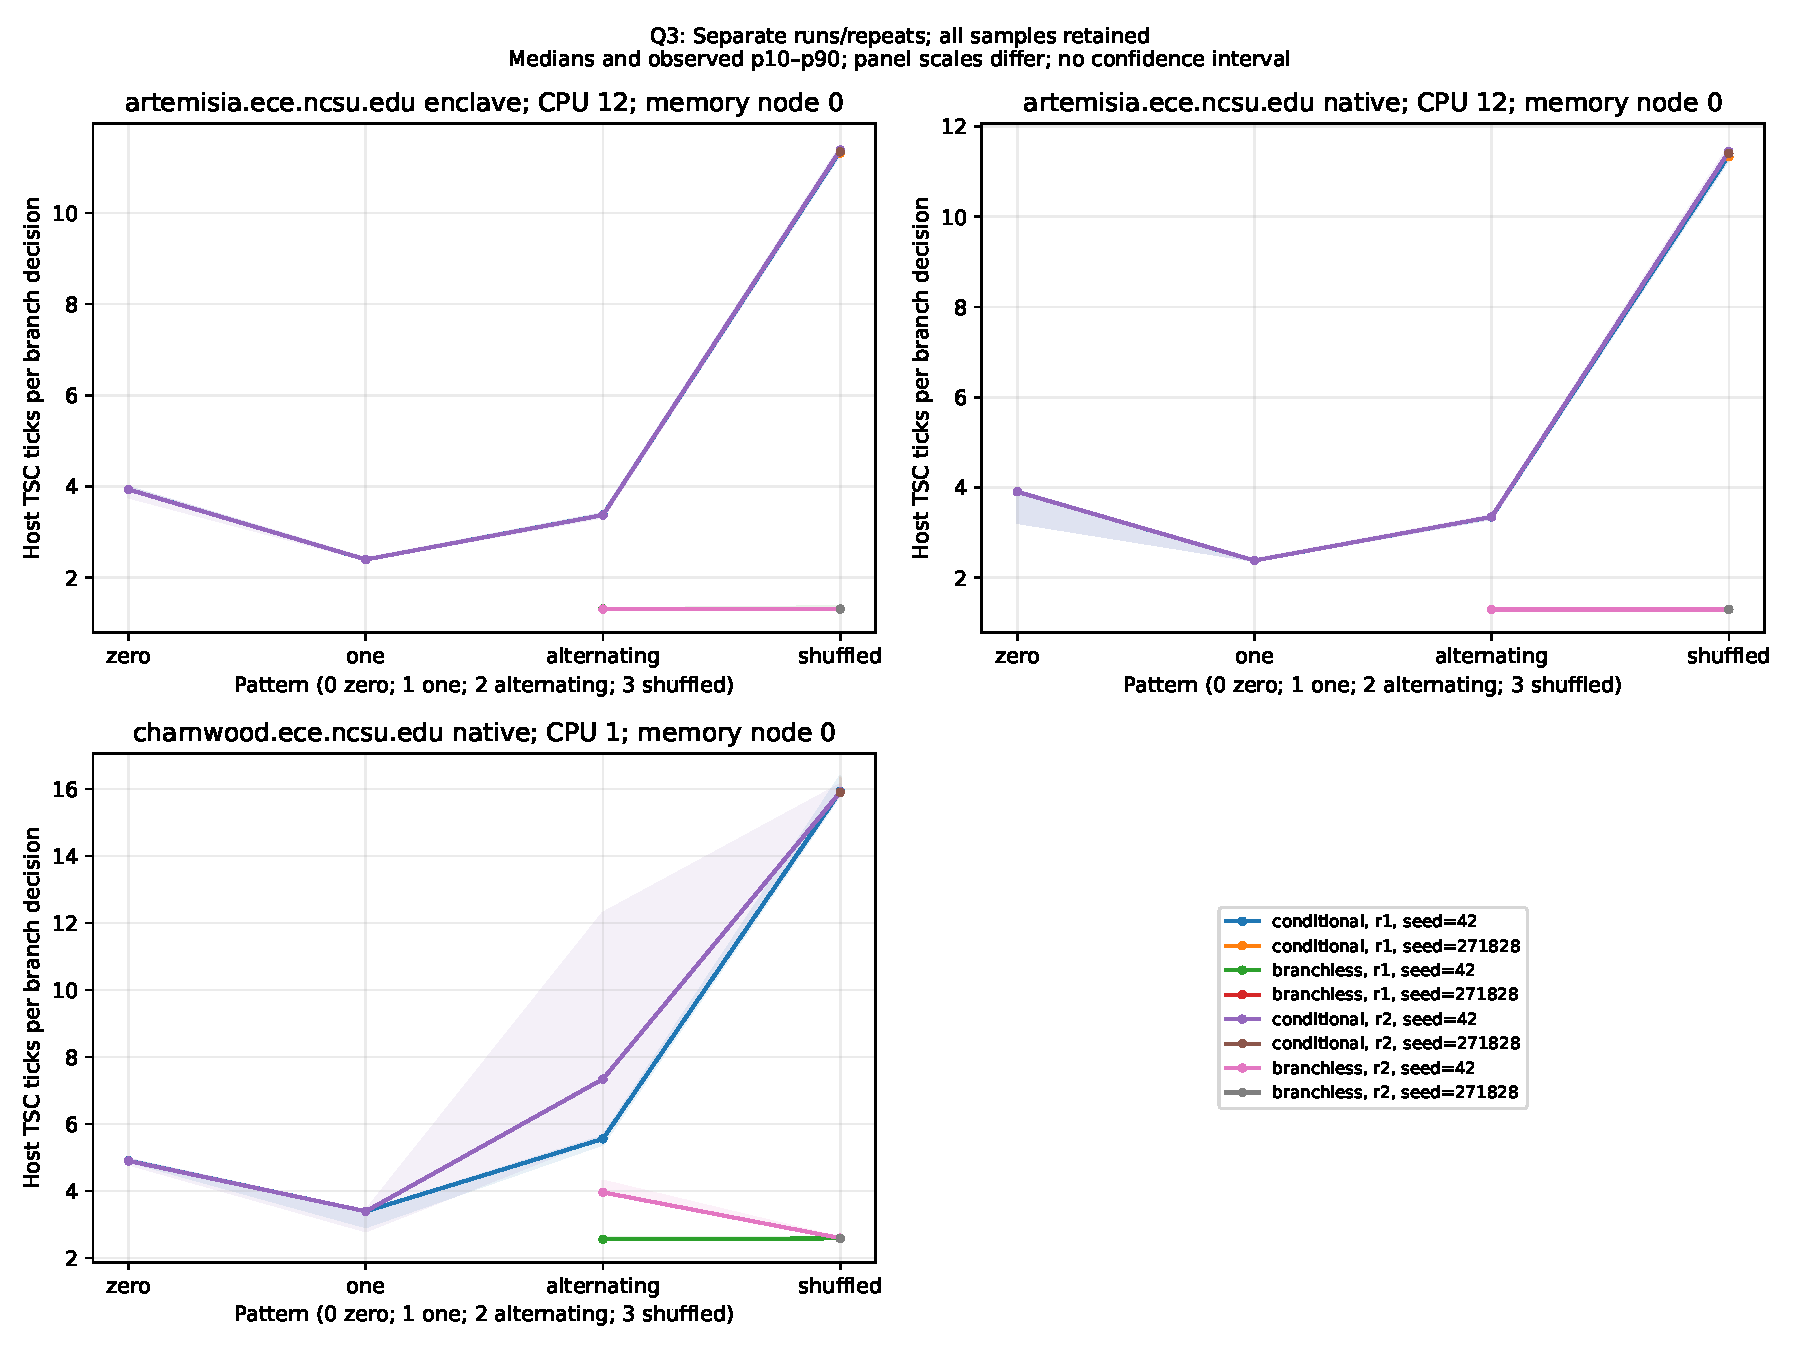
\includegraphics[width=\textwidth]{results/q3-comparison/Q3.pdf}
\caption{Q3 raw TSC comparisons. Each machine has its own tick duration; Charnwood's elapsed-time drift is visible and interpreted using simultaneous native core cycles.}
\end{figure}
Charnwood native alternating conditional work takes 6.0015 / 6.0026 active core cycles/decision, versus 17.6524 / 17.6466 shuffled (seed 42). Branchless alternating is 2.7628 / 2.7640, versus 2.7921 / 2.8002 shuffled; native shuffled branch misses are about 0.496--0.497/decision. Its raw alternating TSC medians drift from 5.5566 to 7.3413 and branchless alternating from 2.5604 to 3.9602, despite stable core-cycle costs. Thus elapsed timing alone would confound the comparison. The cycle and miss evidence supports branch prediction on both CPUs, while the enclave comparison remains timing based. All Charnwood rows are retained in \texttt{results/q3-charnwood-private/}.

\section{Q1: pipelining (10 points)}
The same 32 explicit \texttt{imul \$3,reg,reg} instructions per iteration use one, two or four dependency chains. One chain is latency dominated; multiple chains expose reciprocal throughput. For four chains, the generator emits this group eight times (one chain instead writes R8 for all 32 operations):
\begin{verbatim}
imul $3,%r8,%r8
imul $3,%r9,%r9
imul $3,%r10,%r10
imul $3,%r11,%r11
\end{verbatim}
Each sample executes 100,000 iterations. The 240 retained observations include zero-work invocation controls. Each cell lists the two process medians:
\begin{center}\begin{tabular}{lrrr}
Chains & Native ticks/IMUL & Native cycles/IMUL & SGX ticks/IMUL\\\hline
1 & 2.2314 / 2.2308 & 3.0005 / 3.0005 & 2.2435 / 2.2456\\
2 & 1.1156 / 1.1155 & 1.5003 / 1.5003 & 1.1249 / 1.1251\\
4 & 0.7440 / 0.7435 & 1.0002 / 1.0002 & 0.7500 / 0.7502
\end{tabular}\end{center}
With fixed work, the native dependency latency is about three active core cycles and the initiation interval with independent work about one cycle, a ratio near three. The zero-work medians are 64 native and 11,046 SGX ticks/invocation; no overhead subtraction is applied to the table. They are negligible per IMUL at this batch length. No ordinary faults were recorded; 13 samples had context-switch deltas and remain included.

Multiple execution units are an alternative explanation for independent-work speedup. The selected IMUL form has a single port-1 resource in the separately cited LLVM Skylake/Sapphire Rapids models; this is a reference model, not a measured unit count. The latency/throughput gap together with that resource bound supports pipelined multiplication. Timing alone cannot rule out arbitrary undisclosed replicated hardware or measure whole-CPU pipeline depth. Native core-cycle diagnostics and host TSC ticks are explicitly different units; enclave PMU coverage remains unqualified. Raw data and metadata are in \texttt{results/q1-artemisia/}.
\begin{figure}[htbp]\centering
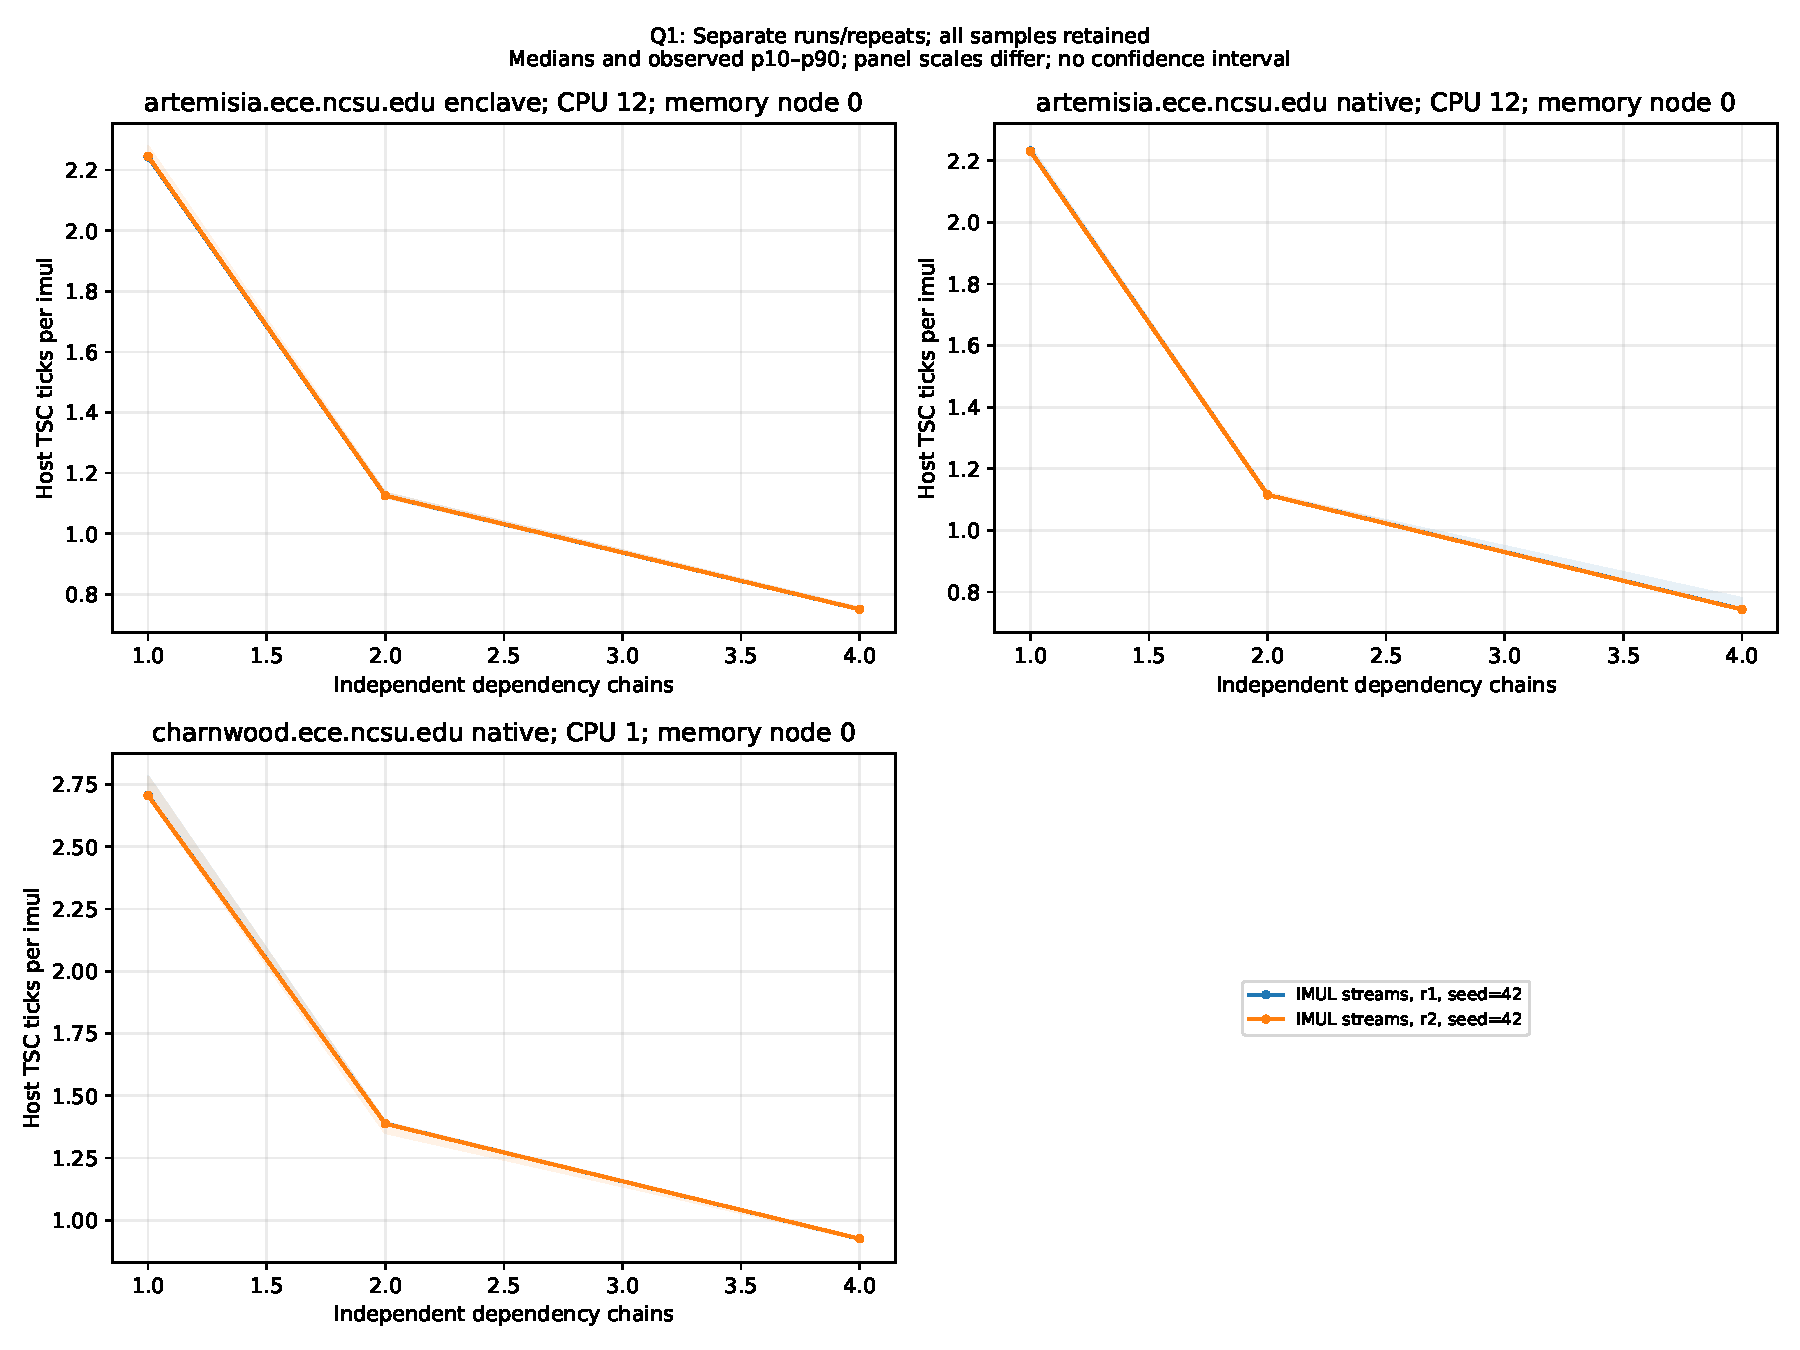
\includegraphics[width=\textwidth]{results/q1-comparison/Q1.pdf}
\caption{Q1 fixed-work dependency experiment on both native machines and Artemisia SGX, with separate repetitions.}
\end{figure}
Charnwood repeats the same native cycle pattern: approximately 3.0006, 1.5003 and 1.0003 core cycles/IMUL for one/two/four chains. Its zero-work median is 76 ticks/invocation in both repetitions. The two CPUs therefore show the same roughly three-cycle dependency latency and one-cycle initiation interval, despite different raw TSC rates. See \texttt{results/q1-charnwood-private/}; the execution-unit replication qualification applies to both machines.

\section{Q2: out-of-order execution (10 points)}
\begin{verbatim}
mov (%r8),%r8          # older pointer load
imul $3,%r8,%rax       # older multiply blocked on load
xor %r11,%r9          # ready source, overlap variant
# K younger imul $3,%r9,%r9 operations
xor %rax,%r10         # consume older result
lfence                # common end-of-block boundary
\end{verbatim}
The dependency-serialized variant uses RAX in the XOR; a third variant inserts LFENCE after the older multiply. All variants end each block with LFENCE to prevent overlap with the next block's load. The randomized cold ring occupies 256 MiB, versus 16 KiB hot; K=0 exposes the baseline and extra fence cost. Each sample has 100,000 blocks. Each cell lists the two process medians, in TSC ticks/block:
\begin{center}\begin{tabular}{lrr}
Treatment & Native & Hardware SGX\\\hline
Cold independent, K=0 & 287.97 / 287.11 & 361.41 / 372.15\\
Cold independent, K=64 & 292.72 / 295.18 & 387.02 / 369.17\\
Cold dependency-serialized, K=64 & 432.31 / 430.24 & 542.05 / 522.43\\
Cold fence-serialized, K=64 & 439.04 / 440.26 & 584.86 / 545.50\\
Hot independent, K=64 & 153.91 / 153.85 & 154.93 / 154.87\\
Hot dependency-serialized, K=64 & 158.44 / 158.58 & 159.52 / 159.50
\end{tabular}\end{center}
Native cold independent work adds only about 5--8 ticks to K=0, while forcing that younger chain to depend on the older blocked multiply adds about 135--140 ticks relative to independent K=64. The independent hot block already takes about 154 ticks, so the cold experiment has substantial work available to hide behind the older load. The extra fence changes cold K=0 by about 9--11 ticks; that overhead is much smaller than the K=64 contrast. The direction also holds inside the enclave, with greater cold timing variation. Given the verified program order, dependency change and common block boundary, this supports younger ready arithmetic executing ahead of the older blocked arithmetic, beyond a claim of independent-stream throughput alone. It is not exact instruction-by-instruction tracing or an additive latency identity.

The accepted campaign \texttt{results/q2-artemisia-retry/} retains 540 observations, zero ordinary faults and 71 samples with context-switch deltas. The preceding partial campaign is preserved separately: its 31st job failed the declared NUMA placement gate, so it is not completed evidence. A pre-implementation pilot without the common end fence is also retained as a rejected assay, not positive OOO evidence.
\begin{figure}[htbp]\centering
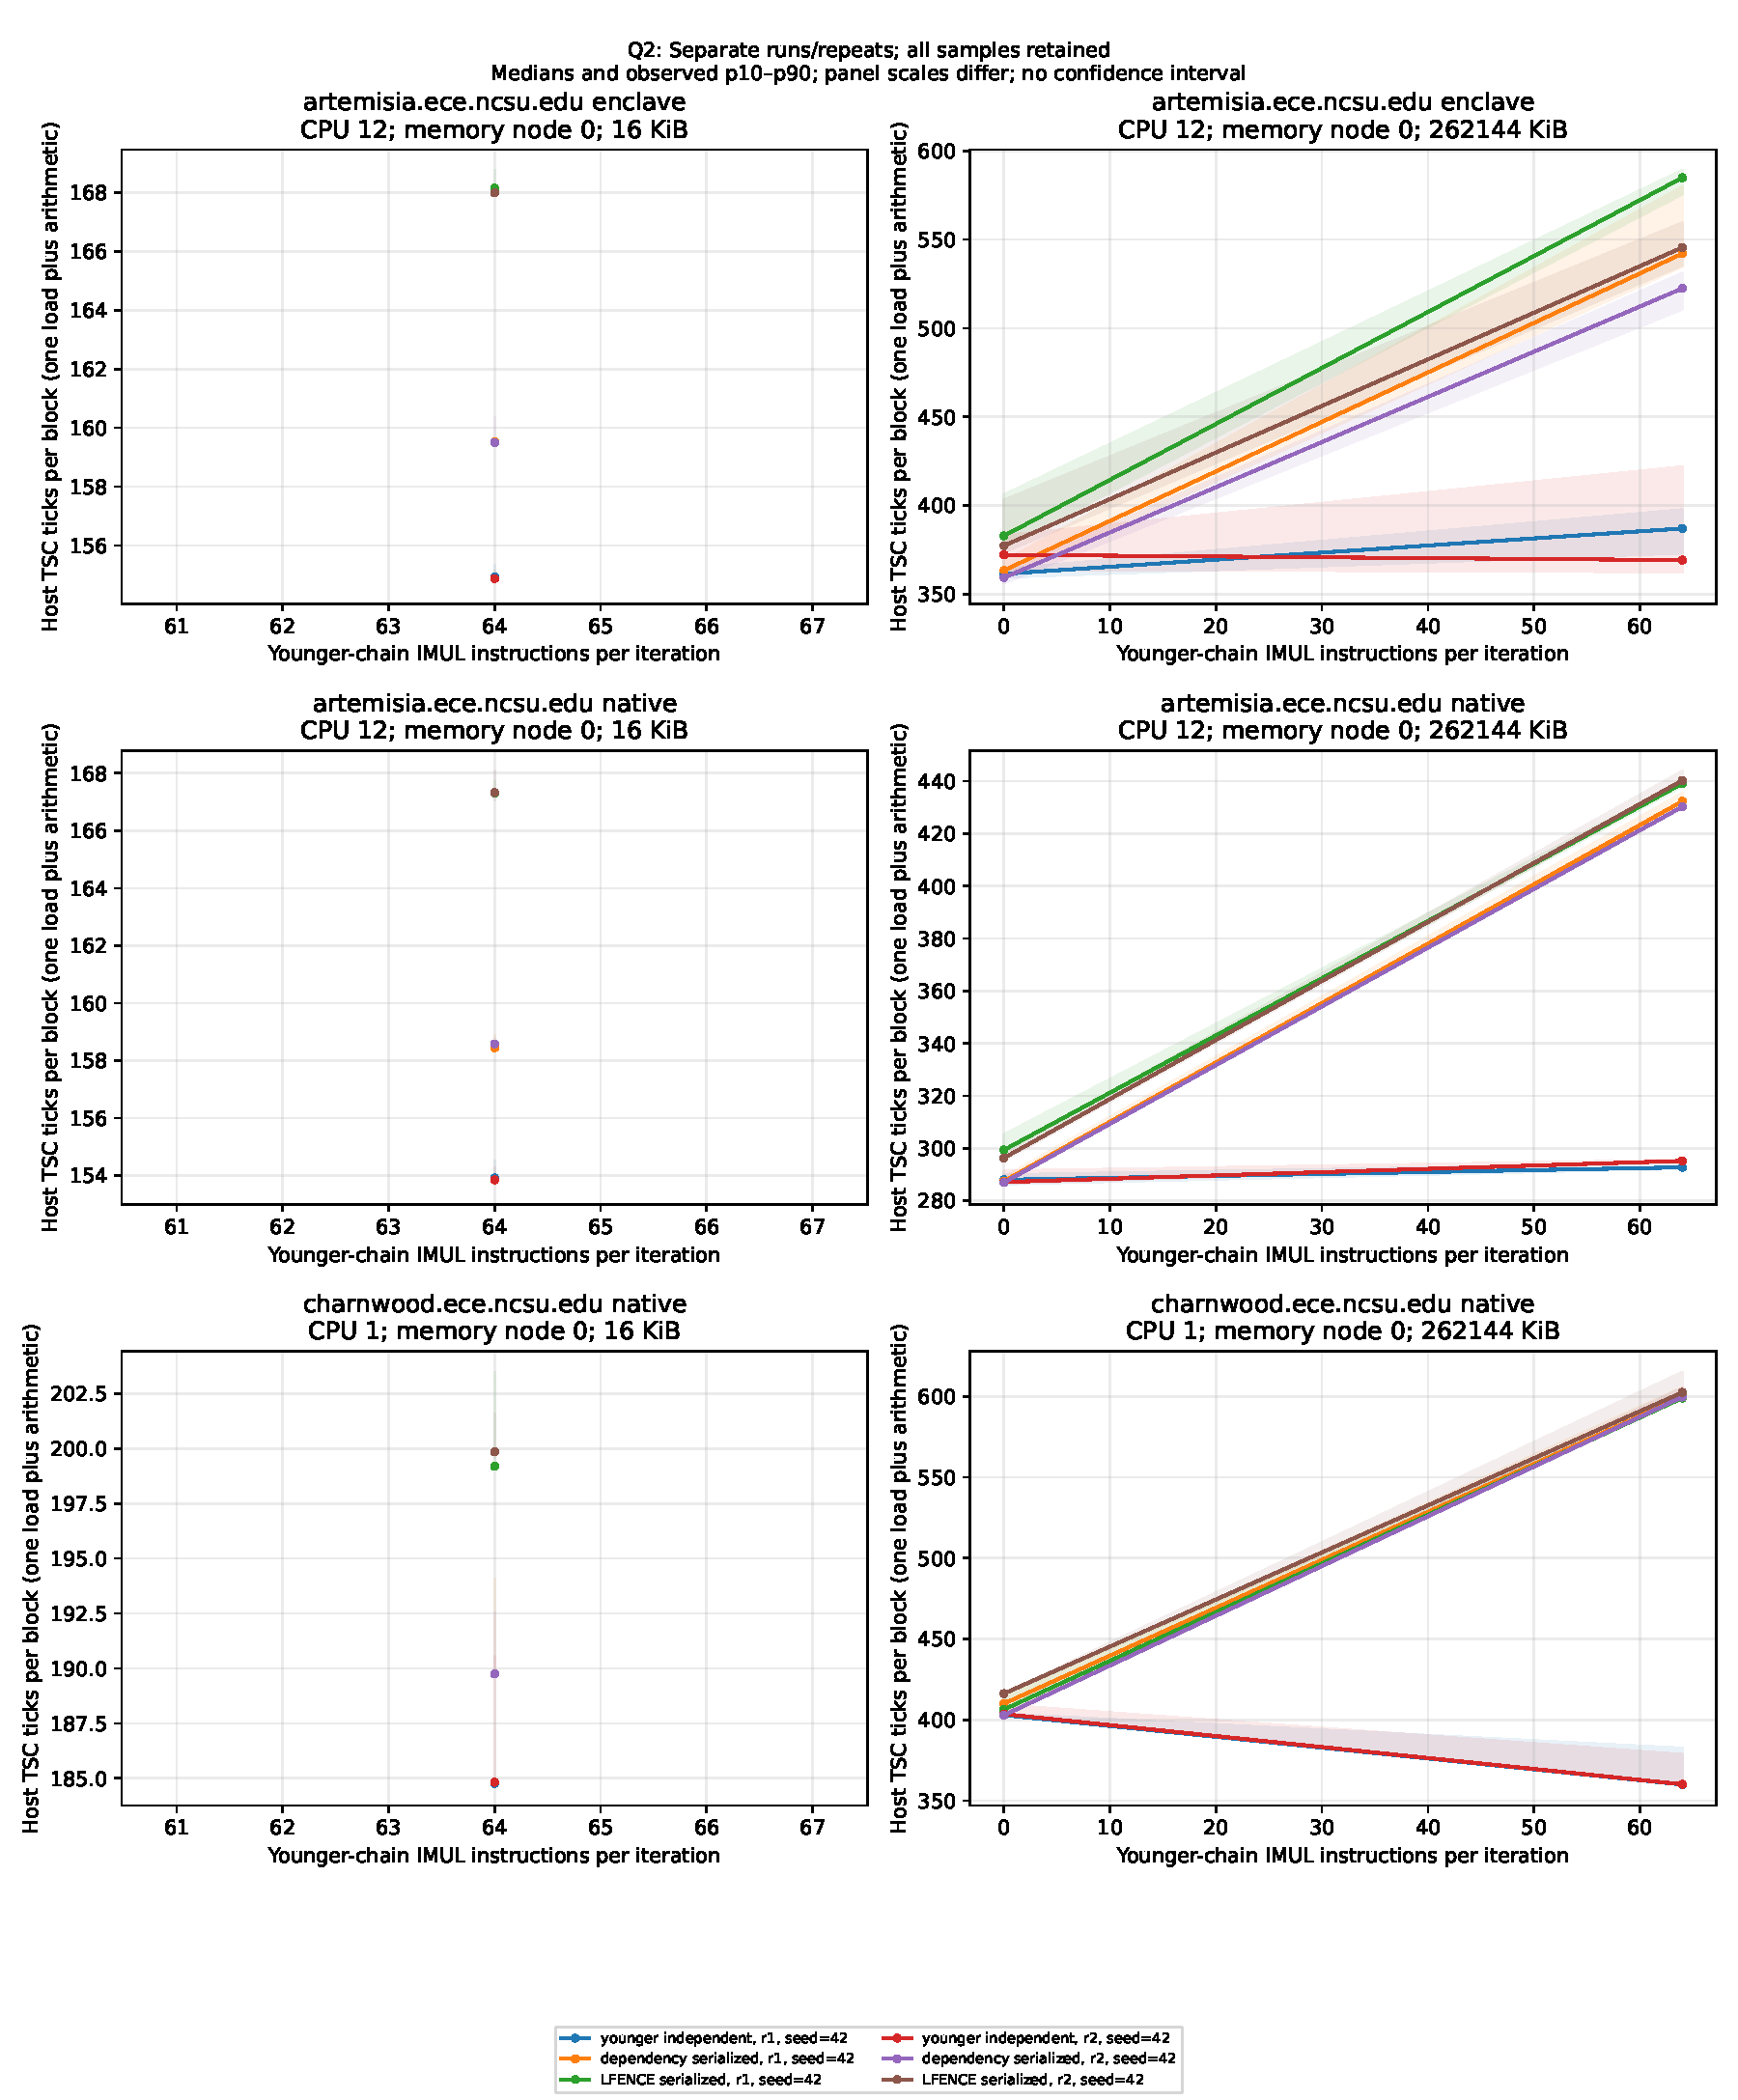
\includegraphics[width=\textwidth]{results/q2-comparison/Q2.pdf}
\caption{Q2 matched dependency/fence controls, separated by machine, environment and hot/cold footprint.}
\end{figure}
Charnwood cold K=64 independent medians are 359.96 / 360.08 ticks/block, versus 599.72 / 599.63 dependency-serialized and 598.99 / 602.43 fence-serialized. Hot independent K=64 is 184.76 / 184.82. This independently supports bypass of the older blocked arithmetic. Its cold K=0 baseline is 402.88 / 403.50, exceeding independent K=64; frequency/memory-state variation prevents exact additive baseline subtraction. The conclusion rests on matched K=64 dependency/fence changes and actual assembly order, not an assumed sum identity. Raw evidence is in \texttt{results/q2-charnwood-private/}.

\section{Q4: preserved completed ROB work (30 points)}
The completed Artemisia evidence is preserved without modification. Two fine campaigns of 1,980 samples each show an effective overlap-loss transition across sampled N=492--500 NOPs per load-to-load gap, in native and hardware-debug SGX builds. It is an operational instruction-window finding; exact total ROB-entry attribution remains qualified in the original analysis. An isolated repeated-enclave N=548 peak is retained and prevents a largest-jump-only estimator from being used blindly.
\begin{center}
\begin{tabular}{rrrrr}
N & Native first & Native repeat & SGX first & SGX repeat\\\hline
492 & 179.55 & 180.02 & 214.67 & 223.14\\
496 & 215.28 & 215.96 & 274.12 & 284.81\\
500 & 288.09 & 289.73 & 365.20 & 368.36
\end{tabular}
\end{center}
Values are independent-load medians in host TSC ticks/load. No raw observations are removed or overhead corrected. The loop has 2N NOPs, two loads and decrement/branch per iteration; neither N nor the entire loop instruction count alone establishes total ROB entries. See the preserved method, controls, raw data and limits in \texttt{ROB\_BENCHMARK.md} and \texttt{ROB\_RESULTS\_ARTEMISIA.md}.
\begin{figure}[htbp]
\centering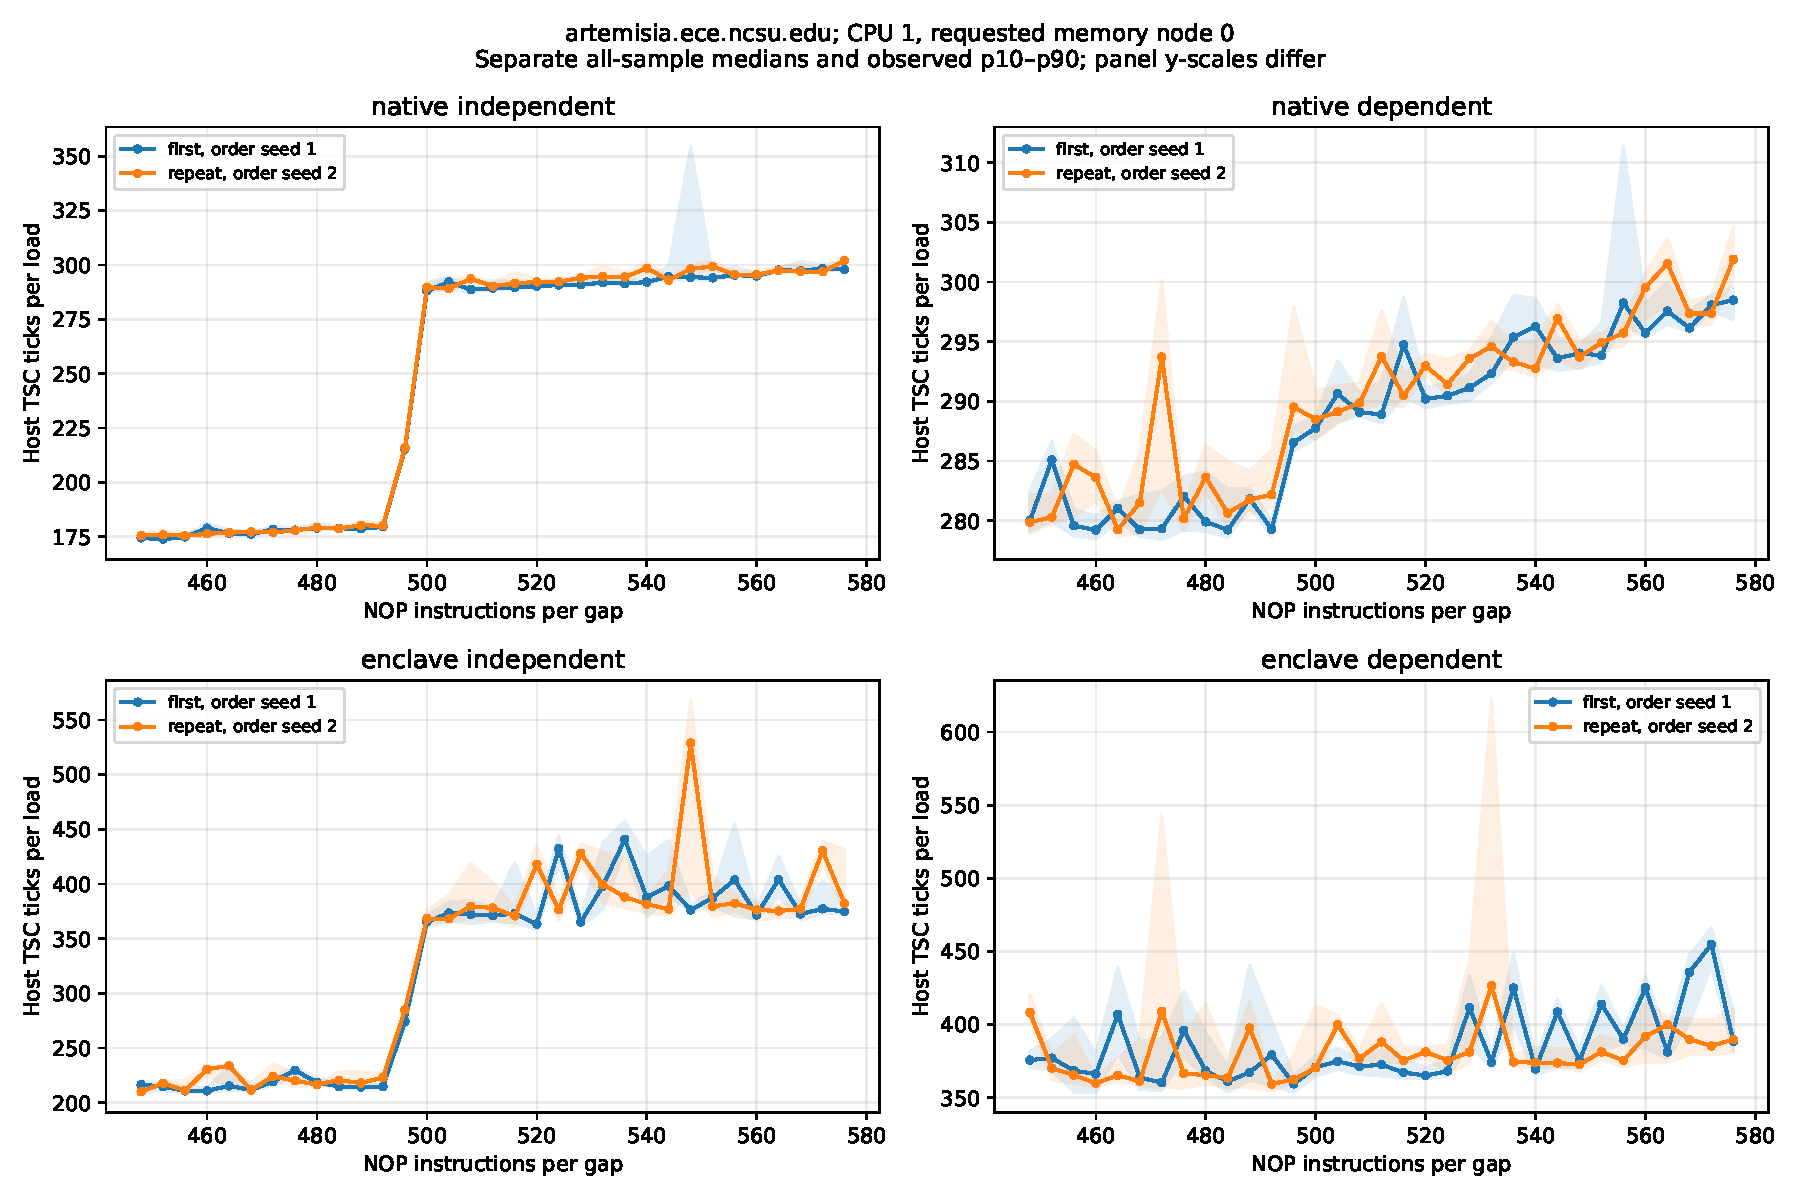
\includegraphics[width=\textwidth]{results/v2-fine-repeat/review/comparison/curves.pdf}
\caption{Preserved Q4 Artemisia fine campaigns. Separate medians and observed p10--p90; panel scales differ. No second-machine curve is synthesized.}
\end{figure}
The user confirmed Charnwood Q4 had not yet been measured. A separate host-local build of the unchanged protected implementation passed its original 3,084-kernel checks and an independent native timer audit. Its build ID remains \texttt{bcd9d621feed36f6}. CPU 1/node 0, a 256 MiB footprint, 100,000 iterations/sample and 15 raw samples/condition match the preserved protocol. A 1,950-observation coarse run selected fine N=192..240; two order-shuffled fine processes retain 390 observations each:
\begin{center}\begin{tabular}{rrr}
N & Independent first / repeat & Serialized first / repeat\\\hline
216 & 282.844 / 284.436 & 389.352 / 389.210\\
220 & 323.444 / 325.026 & 395.995 / 397.681\\
224 & 398.810 / 398.941 & 409.600 / 398.887
\end{tabular}\end{center}
The largest fine step is 220$\rightarrow$224 in both processes, also under minimum and unflagged-median diagnostics; the N=224 ratios are approximately 0.974 and 1.000. This is an effective overlap-loss window, not an asserted total ROB count. Coarse has two faulted observations and 540 with context-switch deltas; fine has zero ordinary faults and 67/75 context-switch observations, all retained. See \texttt{Q4\_CHARNWOOD\_RESULTS.md}. Artemisia's data, figures, analysis and original instructions remain unchanged.
\begin{figure}[htbp]\centering
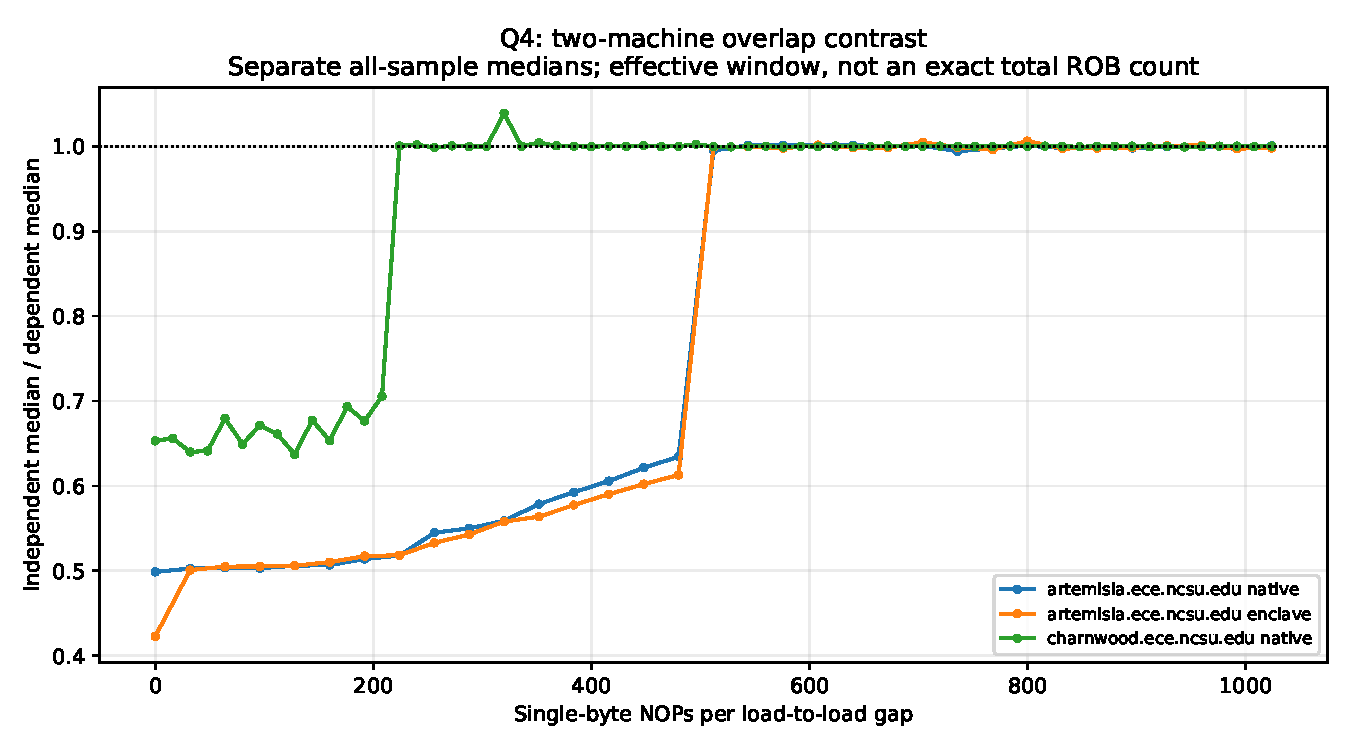
\includegraphics[width=\textwidth]{results/q4-comparison/curves.pdf}
\caption{Q4 within-host median ratios compare overlap without assuming equal TSC duration across machines. Artemisia uses its actual preserved full-range frontend baseline; Charnwood uses its new coarse sweep.}
\end{figure}

\section{Q5: integer physical register allocation (35 points)}
Class: \textbf{64-bit integer GPR}. Replace NOP filler in the two-ring resource-pressure framework with scaled-index \texttt{lea (reg,reg,2),reg}, computing 3*x modulo $2^{64}$. Compare one/four/eight-accumulator variants, a four-byte NOP window control matching instruction count and encoded length, and a serialized-load control. All controls initialize the same eight accumulators and preserve the same callee-saved registers outside the hot loop. The filler has no FLAGS destination, is not a plain move or zero idiom, and avoids pure constant-offset tracking. The oldest delayed load prevents retirement while new destinations accumulate. Execution/scheduler limits remain alternatives if controls disagree.

The first complete 7,920-observation Q5 campaign used constant-offset \texttt{lea 1(reg),reg}. Its one/four-chain curves track NOPs; at N=448, native repetition 2 takes about 468.64 core cycles/iteration despite 896 architectural updates, violating the ordinary one-cycle-chain assumption. The checksum confirms the updates, but their allocation mechanism is unresolved. This campaign is retained as a diagnostic and is not an isolated PRF estimate. Scaled-index results require a separate build and collection.
\begin{verbatim}
loop:
    mov (%rdi),%rdi
    # N actual LEAs: lea (%r8,%r8,2),%r8; rotate registers
    mov (%rsi),%rsi
    # N further LEAs, or N matched four-byte NOPs per gap
    dec %rdx
    jnz loop
\end{verbatim}

The accepted coarse/fine campaigns retain 9,900 and 3,300 observations, respectively, with 10,000 iterations/sample and complete direct native page-node checks. Their broad early transition motivated fine N=192..232 in steps of four. Native fine medians in ticks/load (two process medians per cell) are:
\begin{center}\begin{tabular}{rrrrr}
N & Four chains & Eight chains & NOP & Serialized LEA\\\hline
200 & 168.5 / 171.0 & 164.4 / 163.5 & 142.7 / 143.0 & 276.4 / 276.8\\
204 & 183.2 / 185.9 & 167.5 / 168.2 & 142.7 / 142.7 & 277.4 / 276.8\\
208 & 254.5 / 261.8 & 184.2 / 186.0 & 142.9 / 142.2 & 286.0 / 283.7\\
212 & 273.4 / 276.3 & 278.6 / 272.7 & 142.0 / 142.5 & 286.8 / 287.4\\
216 & 290.3 / 290.6 & 292.2 / 290.0 & 143.3 / 142.4 & 292.6 / 289.5
\end{tabular}\end{center}
Both multi-chain variants lose overlap across approximately N=200--216 and converge near the serialized control, while NOPs remain low and transition only much later in the coarse N=496--512 samples. This separates integer-destination pressure from the NOP instruction-window limit. The onset differs with chain count; one-chain arithmetic is execution-limited earlier, so dependency/scheduler effects remain material. The enclave shows the same broad early transition with more noise: four-chain N=200 is 203.2 / 203.0 ticks/load versus 359.0 / 362.7 at N=216; eight-chain N=200 is 198.0 / 209.8 versus 343.7 / 332.6 at N=212.

The defensible measurement is an \textbf{effective integer-destination pressure window of about 200--216 writes per gap}. Conditional on allocation being the bottleneck, it brackets an operational speculative-allocation budget. Precise PRF-versus-scheduler attribution and the occupancy correction needed for total PRF size remain unresolved. A loop executes 2N LEAs; neither 2N nor N+16 is asserted as total PRF capacity. Committed/live mappings, other in-flight destinations, reclamation and reserved capacity need justified accounting. The coarse campaign retains 22 observations with ordinary faults and 288 with context-switch deltas; fine retains zero faults and 77 context-switch observations. Raw evidence is in \texttt{results/q5-scaled-residency-artemisia/} and \texttt{results/q5-fine-artemisia/}.
\begin{figure}[htbp]\centering
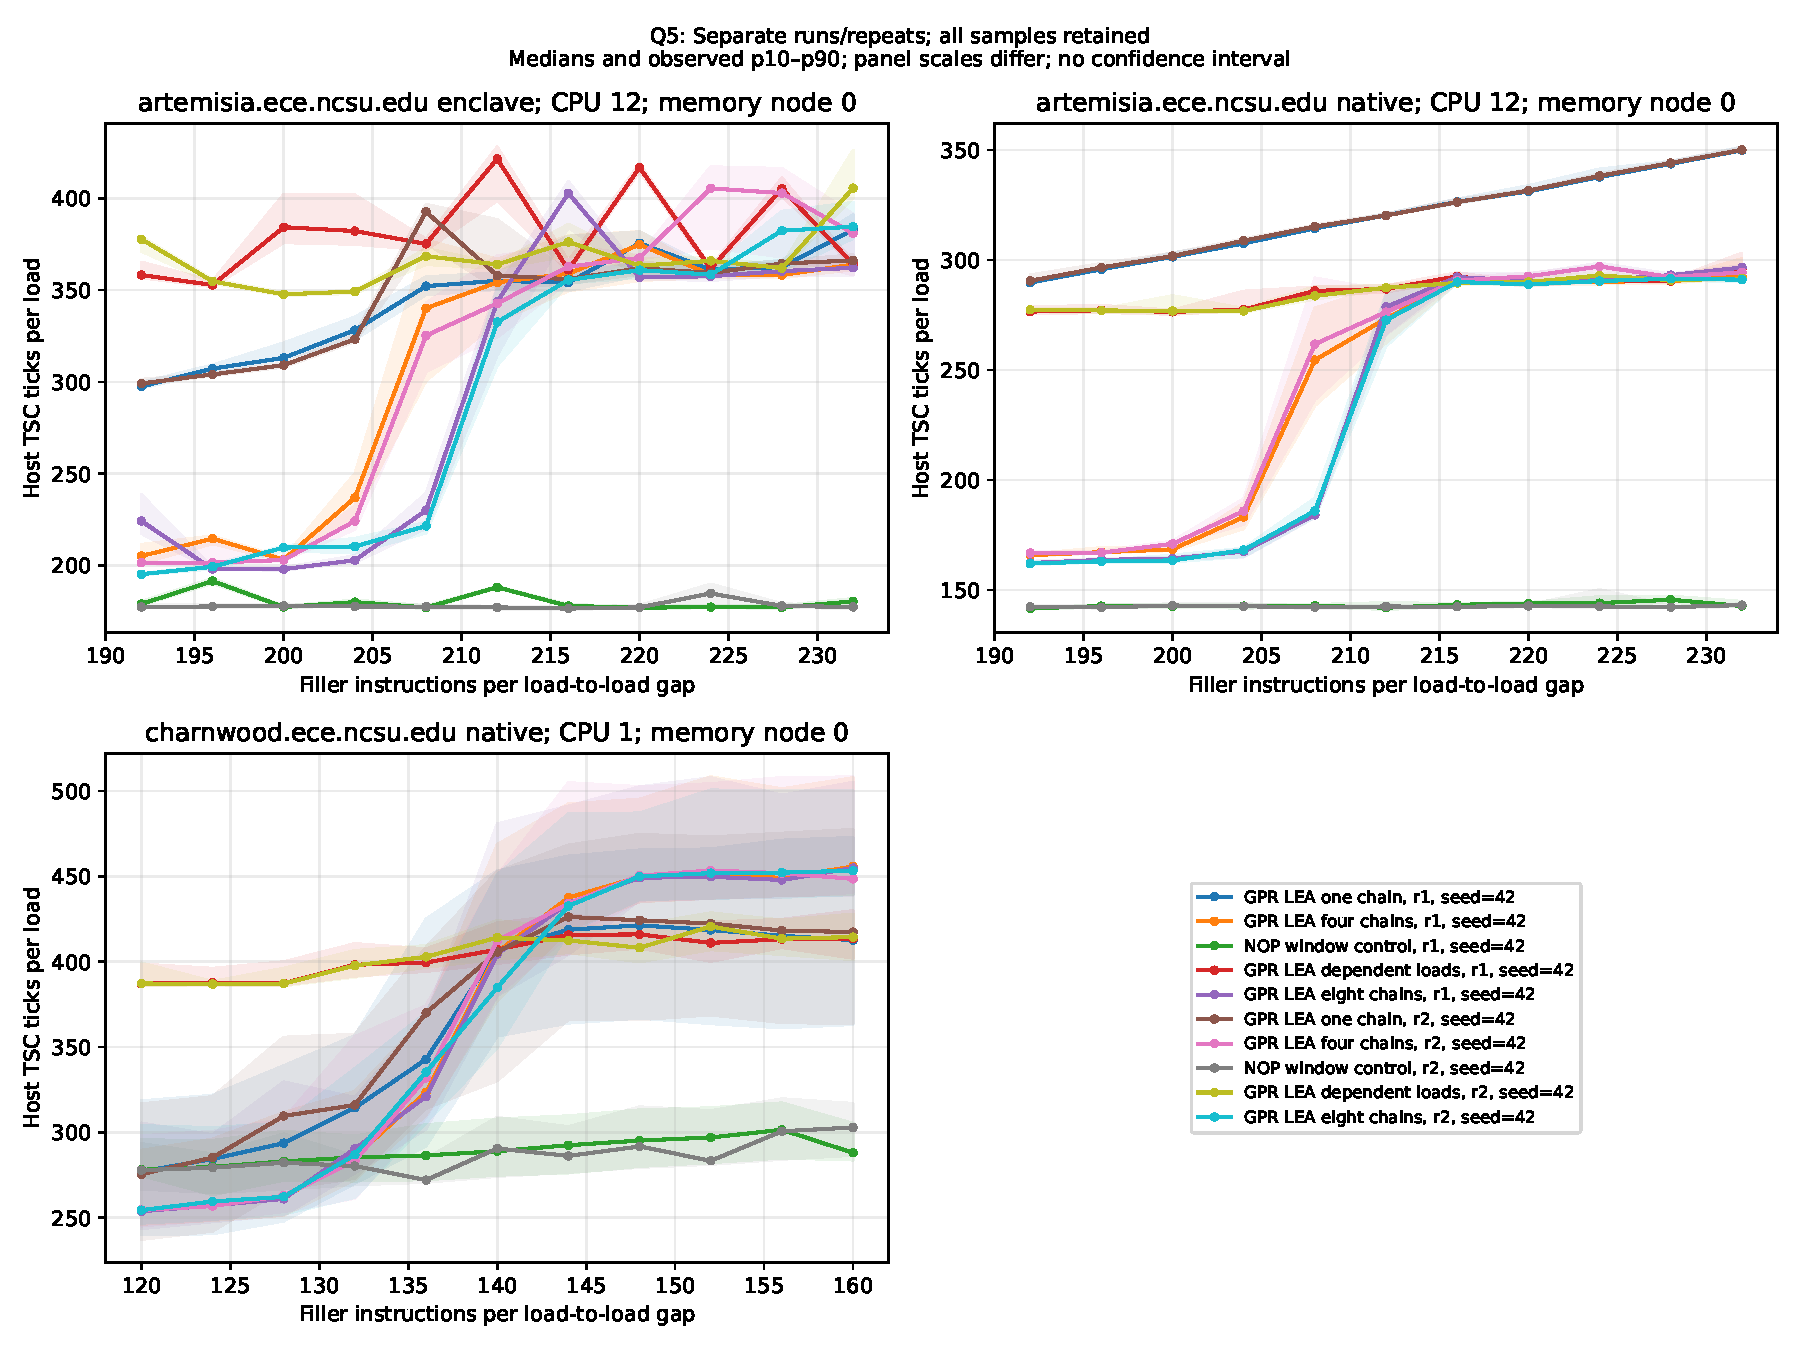
\includegraphics[width=\textwidth]{results/q5-comparison/Q5.pdf}
\caption{Q5 fine intervals selected from each machine's own coarse data. Separate repetitions compare one, four and eight LEA chains with NOP and serialized-load controls.}
\end{figure}
Charnwood's own coarse run selected N=120..160. Four-chain medians rise from 261.90 / 262.83 ticks/load at N=128, to 323.43 / 331.84 at N=136, then 437.49 / 433.96 at N=144. Eight-chain values are 261.03 / 262.23, 320.92 / 335.33 and 434.21 / 432.58, respectively. NOPs remain near 272--292 in this interval and transition later around coarse N=208--224. The effective destination-pressure region is roughly N=128--144, smaller than Artemisia's 200--216 region. Charnwood's post-transition timing can exceed its serialized control, reinforcing that allocation, dependency and scheduler/throughput effects are coupled. The precise PRF-versus-scheduler attribution and total-size conversion remain unproved; neither a published capacity nor a guessed architectural-register correction is substituted.

\section{Q8: additional TLB-miss cost (10 points)}
Target L1 data-TLB misses serviced by the STLB. Compare a compact dependent ring with a scattered one having the same number of cache lines and randomized order. Scattered node i is at \texttt{i*4096+(i\%64)*64}; equal L1-set distribution and 8/16/24 KiB data footprints help retain hot data while changing translation pressure. The baseline is compact translation-resident access.
\begin{verbatim}
loop:
    mov (%r8),%r8
    dec %rsi
    jnz loop
\end{verbatim}
Both native and enclave Q8 arenas are page aligned. Hardware semantic tests check actual arena bases and seed/cursor-derived pointer positions in both layouts, rather than assuming enclave malloc has native page alignment.

Qualified native counters must support additional STLB hits with low completed page walks and low L1D misses, plus at least 98\% group scheduling. A fourth simultaneous counter measures active core cycles. The primary estimate is
\[
\frac{\text{scattered cycles/load}-\text{compact cycles/load}}
{\text{scattered STLB services/load}-\text{compact STLB services/load}}.
\]
This normalizes by observed additional services rather than assuming every load misses. Each sample has 100,000 dependent loads; each cell lists the two process medians' derived costs:
\begin{center}\begin{tabular}{rrr}
Nodes/cache lines & Charnwood extra core cycles & Artemisia extra core cycles\\\hline
128 & 9.0014 / 9.0029 & 7.0016 / 7.0015\\
256 & 9.0052 / 9.0014 & 7.0007 / 7.0023\\
384 & 9.0101 / 9.0043 & 7.0024 / 7.0020
\end{tabular}\end{center}
Both native CPUs pass the miss/cache criteria: additional STLB services exceed 0.5/load, compact service rates are below 0.05/load, recorded 4 KiB walks are zero, and maximum L1D misses/load are 0.00273 on Charnwood and 0.0008 on Artemisia. The supported estimate is therefore \textbf{about 9 additional active core cycles on Charnwood and 7 on Artemisia per L1 data-TLB miss served by the STLB}. It is neither total load latency nor page-walk cost. These cycle counts do not establish nanoseconds across different clock rates; wider-bracket host instructions and event semantics limit precision.

The initial three-event campaign exposed a shifted Charnwood compact baseline (256 nodes, repetition 2: about 6.85 versus 3.70 ticks/load) despite comparable miss/cache rates. It is retained as a diagnostic. Final TSC cost is emitted only when effective cycles/TSC-tick medians match within 2\% and each condition's ratio p90/p10 is at most 1.02. This practical central-80\% clock/preemption check is not proof of fixed frequency or a confidence interval. All Artemisia native pairs pass, yielding about 5.20 extra TSC ticks/service. Four of six Charnwood TSC estimates are withheld for drift/mismatch while their simultaneous core-cycle estimates remain qualified. No individual observation is silently removed.

Final raw collections retain 360 observations on Artemisia (native/enclave) and 180 on Charnwood, with zero ordinary faults and six context-switch observations in each collection. Artemisia enclave compact/scattered medians are approximately 3.83--3.85 versus 9.06--9.44 ticks/load, but protected STLB-event coverage is unqualified. This is a same-machine translation-working-set contrast, not a separately verified enclave TLB-miss penalty. The final manifests are in \path{results/q8-clock-artemisia/} and \path{results/q8-clock-charnwood-private/}. Full hierarchy reconstruction is not selected.
\begin{figure}[htbp]\centering
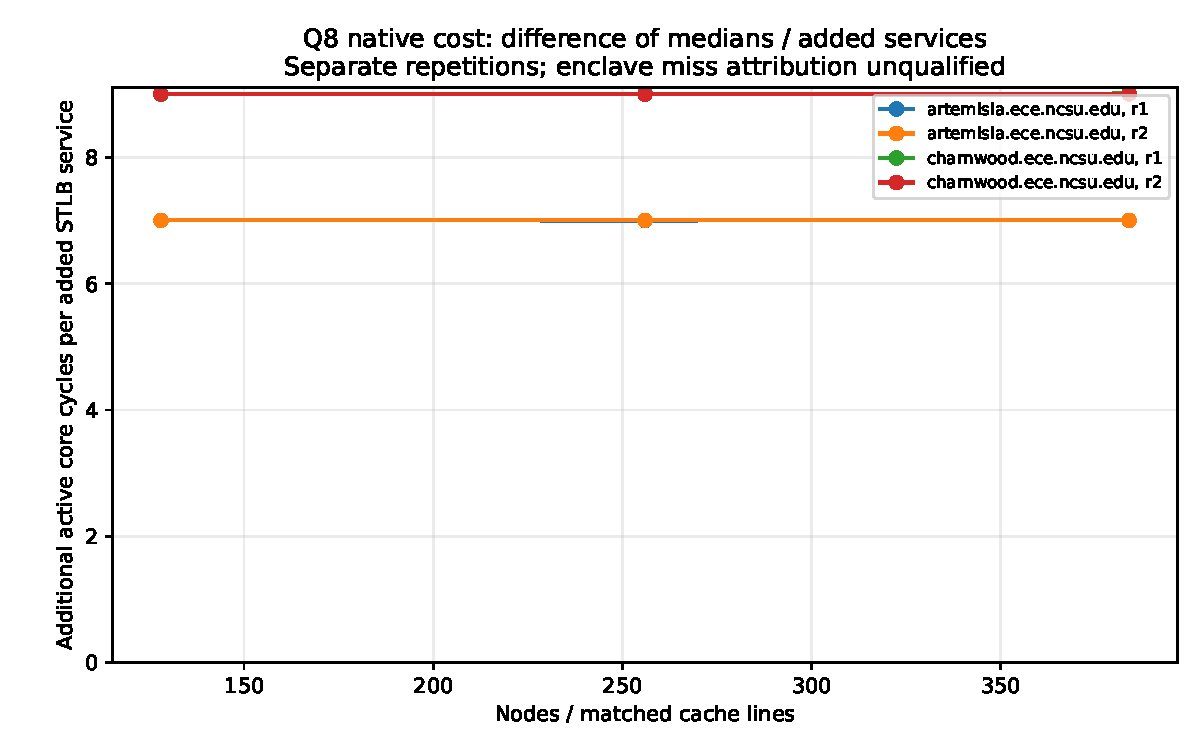
\includegraphics[width=\textwidth]{results/q8-clock-comparison/Q8-cost-core-cycles.pdf}
\caption{Q8 additional native core-cycle cost after compact-baseline subtraction and event-rate normalization; repetitions remain separate. No enclave estimate is invented.}
\end{figure}

\section{Reproduction, limitations and disclosure}
Reproduction commands are in \texttt{README\_Track\_B.md}, \texttt{trackb/METHODS.md} and the preserved Q4 instructions. Raw campaign manifests retain source/binary hashes, exact commands, repetitions, native page/NUMA audits, sibling activity, ordinary disturbances and errors. Smoke data remain functional validation only. Published models/specifications remain separate from measured conclusions. Codex assisted with experiment/code/test design, hardware collection, methodological revisions, analysis, figures and report drafting. All performance rows are actual hardware observations; synthetic formula fixtures are explicitly unit tests. Full chronological assistance is disclosed in AI\_USE\_LOG.md. The accompanying ZIP includes this PDF, source, raw data, figures and plotting scripts, reproduction instructions and the AI-use log. Exact historical builds use each campaign's own source snapshot; current-source reruns are not silently pooled with them. Q4 reproduction uses the protected archive in a separate Charnwood worktree. The report states the remaining scientific attribution limits rather than filling them with published specifications.
\section{Method references}
The following are reference models and interface specifications, separate from measured results:
\begin{itemize}
\item LLVM, \href{https://raw.githubusercontent.com/llvm/llvm-project/main/llvm/lib/Target/X86/X86SchedSkylakeClient.td}{Skylake client scheduling model} and \href{https://raw.githubusercontent.com/llvm/llvm-project/main/llvm/lib/Target/X86/X86SchedSapphireRapids.td}{Sapphire Rapids scheduling model}, for the selected IMUL resource model.
\item Intel, \href{https://www.intel.com/content/dam/www/public/us/en/documents/manuals/64-ia-32-architectures-software-developer-vol-2a-manual.pdf}{Instruction reference, Volume 2A}, for LFENCE ordering.
\item Intel PerfMon, \href{https://raw.githubusercontent.com/intel/perfmon/main/SKL/events/skylake_core.json}{Skylake events} and \href{https://raw.githubusercontent.com/intel/perfmon/main/SPR/events/sapphirerapids_core.json}{Sapphire Rapids events}, for Q8 event definitions.
\item Linux, \href{https://man7.org/linux/man-pages/man2/perf_event_open.2.html}{perf\_event\_open interface}, for counting groups and scheduling coverage.
\item Linux, \href{https://docs.kernel.org/admin-guide/hw-vuln/core-scheduling.html}{core scheduling}, for inherited private task groups and their kernel/interrupt limits; \href{https://man7.org/linux/man-pages/man2/move_pages.2.html}{move\_pages}, for read-only per-page node queries.
\end{itemize}
\end{document}
